\documentclass{article}
\usepackage[LGR,T1]{fontenc}
\usepackage[utf8]{inputenc}
\usepackage[greek, english]{babel}
\usepackage{alphabeta}
\usepackage{natbib}
\usepackage{graphicx}
\usepackage{biblatex}
\addbibresource{references.bib}

\def\code#1{\texttt{#1}}

\usepackage{eso-pic}% http://ctan.org/pkg/eso-pic
\usepackage{lipsum}% http://ctan.org/pkg/lipsum

\title{Use Cases - v0.3}

\author{\\

\includegraphics[width=3in]{safeguard}\\[1ex]\\\\
}

\begin{document}

\maketitle

\newpage

\noindentΌλα τα μέλη της ομάδας συνεισέφεραν σε αυτό το έγγραφο.\\

\begin{tabular}{|l|c|c|}
\hline
Όνοματεπώνυμο & email & Αριθμός μητρώου  \\
\hline
Θεόδωρος Ντάκουρης & ntakouris@ceid.upatras.gr & 1054332 \\
Βασίλειος Βασιλόπουλος & vvasil@ceid.upatras.gr &  1054410 \\
Νικόλαος Σουλτάνης & soultanis@ceid.upatras.gr & 1054319  \\
Βάιος Λασκαρέλιας & laskarelias@ceid.upatras.gr & 1054432 \\
Αντόν Πάπα & papa@ceid.upatras.gr & 1054337 \\
\hline
\end{tabular}

\renewcommand{\contentsname}{Περιεχόμενα}
\tableofcontents

\newpage

\section{Αλλαγές}
\subsection{v0.2}
\begin{itemize}
    \item Σε γενικές γραμμές, έχουν γίνει μεγάλες αλλαγές, όπως η μετακίνηση του καθενός use case σε ολοκληρωμένο γράφημα και όχι ξεχωριστά, καθώς και αναθεώρηση όλων τον σχέσεων σε όλες τις περιπτώσεις
    \item Αλλάχτηκαν δραστικά όλες οι περιγραφές ώστε να φαίνεται ο actor σε κάθε βήμα και να υπάρχει σχεδόν παντού ενεργητική φωνή
    \item Εάν διαβάζετε το v0.2 και έχετε διαβάσει το v0.1 θα πρέπει να κοιτάξετε το διάγραμμα από την αρχή
    \item Στο Check In-Out άλλαξε ο Actor από RFID Card Reader σε 'Human Entity'. Προστέθηκαν λίγες λεπτομέρειες στις εναλλακτικές ροές αυξάνοντας την σαφήνεια των περιγραφών.
    \item Άλλαξε ελάχιστα η βασική ροή στο insert-delete employee
    \item Στο incident submission άλλαξαν οι Actors 
    \item Προστέθηκε μία ακόμα εναλλακτική ροή στο Drone Notifications που προέκυψε απο το Robustness analysis.
    \hline 
    \item Μετονομασία Pin entry ή pin confirmation σε pin authorization για λόγους naming consistency.
\end{itemize}
\subsection{v0.3}
\begin{itemize}
    \item Έγινε επανεγγραφή της ροής του Send Drone, με μεγαλύτερη σαφήνεια.
\end{itemize}

\section{Περιγραφές}

\subsection{RFID Check In-Out}

\noindent Βασική ροή:
\begin{itemize}
    \item Ο εργαζόμενος χτυπάει την κάρτα του
    \item Το σύστημα διαβάζει την κάρτα
    \item Έλεγχοι: 
    \begin{itemize}
        \item Το σύστημα ελέγχει τον σωστό τύπο εισόδου (security - guest - employee)
        \item Το σύστημα ελέγχει εάν έχει βάρδια ο εργαζόμενος
        \item Το σύστημα επιβεβαιώνει ότι δεν έχει λήξει η κάρτα 
        \item Το σύστημα ελέγχει ότι ο εργαζόμενος εισέρχεται σε σωστό πόστο-περιοχή εισόδου
    \end{itemize}
    \item Το σύστημα παίζει έναν χαρακτηριστικός υψίτονο ήχο επιτυχίας
    \item Το σύστημα γράφει το συμβάν σε κάποιο μέσο μόνιμης αποθήκευσης για να υπάρχει αρχείο με τα συμβάν.
    \item Το σύστημα εμφανίζει στον security guy μήνυμα επιτυχημένης εισόδου ως ειδοποίηση
\end{itemize}

\noindent Εναλλακτική ροή 1: 
\begin{itemize}
    \item Το σύστημα διαπιστώνει πως κάποιος από τους παραπάνω ελέγχους αποτυγχάνει.
    \item Αποθηκεύεται αυτή η αποτυχία στο μέσο μόνιμης αποθήκευσης
    \item Το σύστημα εμφανίζει στον security guy μήνυμα λάθους ως ειδοποίηση
    \item Το σύστημα παίζει ο ήχος αποτυχίας
\end{itemize}

\noindent Εναλλακτική ροή 2: 
\begin{itemize}
    \item Το σύστημα διαπιστώνει πως υπάρχει λάθος κατά την ανάγνωση της κάρτας
    \item Το σύστημα εμφανίζει στον security guy μήνυμα λάθους ως ειδοποίηση
\end{itemize}

\noindent Εναλλακτική ροή 3: 
\begin{itemize}
    \item Σε περίπτωση που ο εργαζόμενος κάνει check out,
    \item Το σύστημα ελέγχει και εάν έχει γίνει προηγουμένως check in από τον εργαζόμενο
    \item η ροή συνεχίζει μετά τους ελέγχους
\end{itemize}

\noindent Περαιτέρω εξήγηση:
\begin{itemize}
\item RFID Check In = RFID Basic Access Check
\item RFID Check Out = RFID Basic Access Check + Εάν έχει κάνει σωστά check in ο εργαζόμενος
\end{itemize}

\subsection{Insert-Delete Employee}

\noindent Βασική ροή:
\begin{itemize}
    \item Ο security guy εισάγει τα παρακάτω δεδομένα που απαιτούνται για την έκδοση κάρτας.
    \begin{itemize}
        \item Employee ID
        \item Κάρτα RFID
        \item Ονοματεπώνυμο
        \item Access Level
        \item Expiry Date
    \end{itemize}
    \item Επίσης προαιρετικά εισάγει λόγο διαγραφής - εγγραφής 
    \item καθώς και έγγραφου από γραμματεία - HR
    \item Το σύστημα διαβάζει την κάρτα RFID
    \item Ο security guy εισάγει το πιν του για να πραγματοποιήσει pin authorization
    \item Το σύστημα εκδίδει ή καταστρέφει τα δεδομένα της κάρτας εισόδου
    \item Το σύστημα σημειώνει την εγγραφή-διαγραφή της κάρτας στα access logs.
\end{itemize}

\noindent Εναλλακτική ροή 1: 
\begin{itemize}
    \item Το σύστημα διαπιστώνει πως ο security guy προσπαθεί να κάνει εισαγωγή εργαζομένου με ID που υπάρχει ήδη
    \item Το σύστημα εμφανίζει μήνυμα λάθους και επαναλαμβάνεται η διαδικασία
\end{itemize}

\noindent Εναλακτική ροή 2:
\begin{itemize}
    \item Το σύστημα διαπιστώνει πως η κάρτα RFID ανήκει σε άλλον / δεν έχει διαγραφεί σωστά / είναι corrupted / έχει χαλάσει ολοκληρωτικά
    \item Το σύστημα εμφανίζει μήνυμα λάθους
    \item Το σύστημα σβήνει και απενεργοποιεί την κάρτα
    \item Ο security guy επαναλαμβάνει τη διαδικασία με νέα κάρτα (από τη στοίβα που έχει στο γραφείο του)
\end{itemize}

\noindent Εναλλακτική ροή 3:
\begin{itemize}
    \item Το σύστημα διαπιστώνει πως γίνεται εγγραφή κάποιου εργαζομένου που υπάρχει ήδη
    \item Το σύστημα εμφανίζεται μήνυμα λάθους και επαναλαμβάνεται η διαδικασία
\end{itemize}

\noindent Εναλλακτική ροή 4:
\begin{itemize}
    \item Ο security guy επιλέγει να εισάγει guest.
    \item Το σύστημα δεν κάνει τους ελέγχους για τα δεδομένα που σχετίζονται με τον employee
    \item Εκδίδεται μια προσωρινή κάρτα
\end{itemize}


\subsection{Browse Access Logs}

\noindent Βασική ροή:
\begin{itemize}
    \item Το σύστημα προβάλει τα τελευταία incident στην οθόνη
    \item O security guy εισαγάγει (προαιρετική) κάποια απο τα φίλτρα αναζήτησης:
    \begin{itemize}
        \item incident type (alarm / check in-out / security incident)
        \item incident ID
        \item χρονικές περιόδους
        \item RFID κάρτα εργαζομένου
    \end{itemize}
    \item Το συστήμα προβάλλει στο UI τα αποτελέσματα
\end{itemize}

\noindent Εναλλακτική ροή 1:
\begin{itemize}
    \item Το συστημα δεν εμφανίζει κανένα incident
\end{itemize}

\noindent Εναλλακτική ροή 2:
\begin{itemize}
    \item Το access log έχει καταστραφεί
    \item Το σύστημα εμφανίζει μήνυμα για επικοινωνία με τεχνική υποστήριξη
\end{itemize}

\subsection{Drone notifications}

\noindent Βασική ροή:
\begin{itemize}
    \item Το Drone αναγνωρίζει πιθανούς παράγοντες συναγερμού: (προαιρετικά)
    \begin{itemize}
        \item άτομα
        \item ζώα 
        \item φωτιά
        \item μηχανοκίνητα οχήματα
    \end{itemize}
    \item Το drone εκμπέμπει video livestream 
    \item Κάνει λήψη, αποθήκευση και αποστολή φωτογραφιών
    \item Κατά τη λήξη, ξεκινάει διαδικασία incident submission στον security guy
\end{itemize}

\noindent Εναλλακτική ροή 1:
\begin{itemize}
    \item Αποτυχία σύνδεσης με κέντρο ελέγχου
    \item Αυτόματο recall
    \item Ειδοποίηση μόλις αποκατασταθεί η σύνδεση
\end{itemize}

\noindent Εναλλακτική ροή 2:
\begin{itemize}
    \item Inactivity για παραπάνω από 2 λεπτά στην τοποθεσία συμβάντος
    \item Αυτόματο recall
\end{itemize}
\noindent Εναλλακτική ροή 3:
\begin{itemize}
    \item Δεν αναγνωρίστηκε κανένας τύπος incident
    \item Αυτόματο Recall
\end{itemize}


\subsection{Incident Submission}

\noindent Βασική ροή:
\begin{itemize}
    \item Το Drone ή το Perimeter Monitoring System απαιτούν από τον αρμόδιο security guy να αρχίσει τη διαδικασία καταχώρησης περιστατικού (μπορεί όμως και ο ίδιος ο security guy να αρχίσει τη διαδικασία από το κεντρικό μενού)
    \begin{itemize}
        \item Το σύστημα κάνει αυτόματη εισαγωγή της τρέχουσας ώρας
        \item Ο αρμόδιος actor κάνει εισαγωγή του θέματος κύριου συμβάντος
        \item Ο αρμόδιος actor κάνει εισαγωγή επιπλέων σχολίων
    \end{itemize}
    \item Ο security guy κάνει pin authorization
    \item Το σύστημα κάνει αποθήκευση της τελικής έκδοσης του συμβάντος
\end{itemize}

\noindent Εναλλακτική ροή 1:
\begin{itemize}
    \item Ο security guy κάνει αποτυχημένο pin authorization
    \item To σύστημα στέλνει ανώνυμο report με όλα τα στοιχεία που υπάρχουν διαθέσιμα στα κεντρικά (ώστε να εξεταστεί “χειροκίνητα” το συμβάν)
\end{itemize}

\subsection{Send drone}
% todo: vaios
\noindent Βασική ροή:
\begin{itemize}
    \item Η κάμερα ή ο αισθητήρας στέλνει ειδοποίηση για συγκεκριμένο συμβάν
    \item Το Perimeter Monitoring System εντοπίζει και καταγράφει την τοποθεσία του συμβάντος
    \item Το Perimeter Monitoring System αποστέλλει το drone για αποστολή εξερεύνησης (εκκινείται το use case “drone notifications”)
    \item Το σύστημα ειδοποιεί το Central Office για το περιστατικό
    \item Ο Security Guy έχει την δυνατότητα επιλογής ανάκλησης του Drone
    \item Εκκινείται το use case “Incident Submission” για να αναλάβει την καταχώρηση των περιστατικών με περαιτέρω σχόλια από τον Security Guy
\end{itemize}

\noindent Εναλλακτική ροή 1:
\begin{itemize}
    \item Ο Security Guy επιλέγει να μην σταλεί το Drone
\end{itemize}

\noindent Εναλλακτική ροή 2:
\begin{itemize}
    \item Το drone δεν μπορεί να ξεκινήσει την πτήση ή παρουσιάζει πρόβλημα κατά τη διάρκεια πτήσης
    \item Επιχειρούμε αυτόματο recall εάν δύναται
    \item Το σύστημα ειδοποιεί το Central Office για την τοποθεσία του drone στα κεντρικά (αν δεν γίνει recall)
    \item Εκκινείται το Use case “Incident Submission”
\end{itemize}

\subsection{Silent alarm}

\noindent Βασική ροή:
\begin{itemize}
    \item O Security Guy εισάγει περιγραφή (προαιρετικά)
    \item O Security Guy εισάγει το PIN του
    \item Το σύστημα ειδοποιεί το Central Office για το περιστατικό
\end{itemize}

\subsection{pin authorization}

\noindent Βασική ροή
\begin{itemize}
    \item (Το σύστημα εμφανίζει στον χρήστη αίτημα για εισαγωγή pin και έγκριση διαδικασίας)
    \item Ο security guy εισάγει το PIN του
    \item Έλεγχοι:
    \begin{itemize}
        \item Το σύστημα ελέγχει αν το PIN είναι σωστό και αντιστοιχεί στον εργαζόμενο που δουλεύει εκείνη τη στιγμή.
    \end{itemize}
    \item Ο security guy επιβεβαιώνει την έγκριση διαδικασίας 
    \item (Το σύστημα επιστρέφει στην προηγούμενη διαδικασία)
\end{itemize}

\noindent Εναλλακτική ροή 1:
\begin{itemize}
    \item Ο security guy ακυρώνει τη διαδικασία
    \item (Το σύστημα επιστρέφει στην προηγούμενη διαδικασία απουχημένα)
\end{itemize}

\noindent Εναλλακτική ροή 2:
\begin{itemize}
    \item Ο security guy βάζει το PIN λανθασμένα λιγότερες από 3 φορές
    \item Το σύστημα επιτρέπει έως 3 φορές προσπάθεια εισόδου PIN.
    \item Αν τελειώσουν οι προσπάθειες το σύστημα στέλνει ειδοποίηση στα κεντρικά για λανθασμέν χρήης του PIN
    \item Το σύστημα εμφανίζε παράλληλα και μήνυμα για το πόσες προσπάθειες έχουν απομείνει
    \item (Το σύστημα επιστρέφει στην προηγούμενη διαδικασία αποτυχημένα)
\end{itemize}

\noindent Εναλλακτική ροή 3:
\begin{itemize}
    \item Ο security guy εισάγει το PIN λανθασμένα 3 φορές
    \item Το σύστημα στέλνει μήνυμα στα κεντρικά γραφεία για κακή χρήση του PIN
    \item (Το σύστημα επιστρέφει στην προηγούμενη διαδικασία αποτυχημένα)
\end{itemize}

\section{Διάγραμμα}

Για δική σας ευκολία παρακαλώ να δείτε πέρα από τα screenshots το παρακάτω view-only link από draw.io:

\url{https://drive.google.com/file/d/1T96uwhriuCEeYI0NFlSMREWsfzCgKjQs/view?usp=sharing}
\\
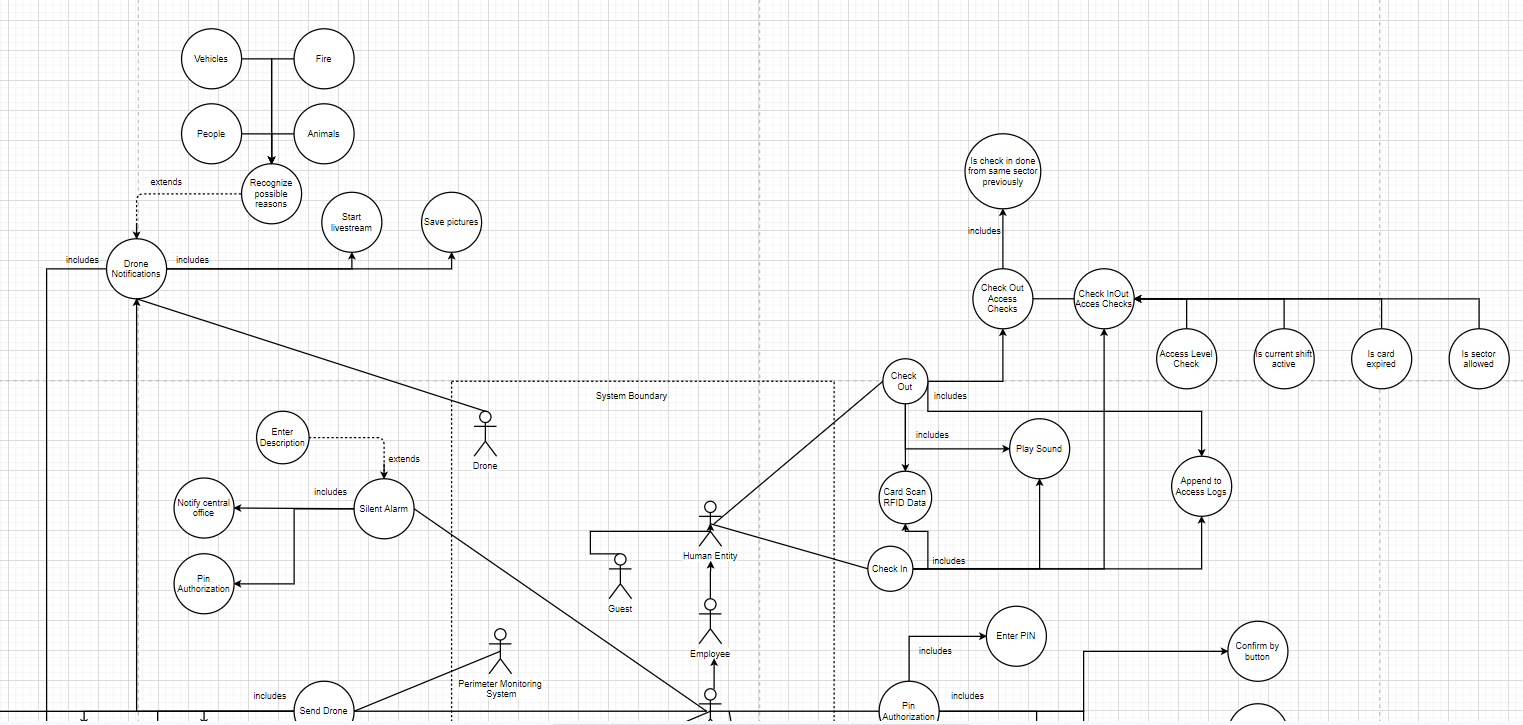
\includegraphics[width=5in]{use1}\\[1ex]\\\\
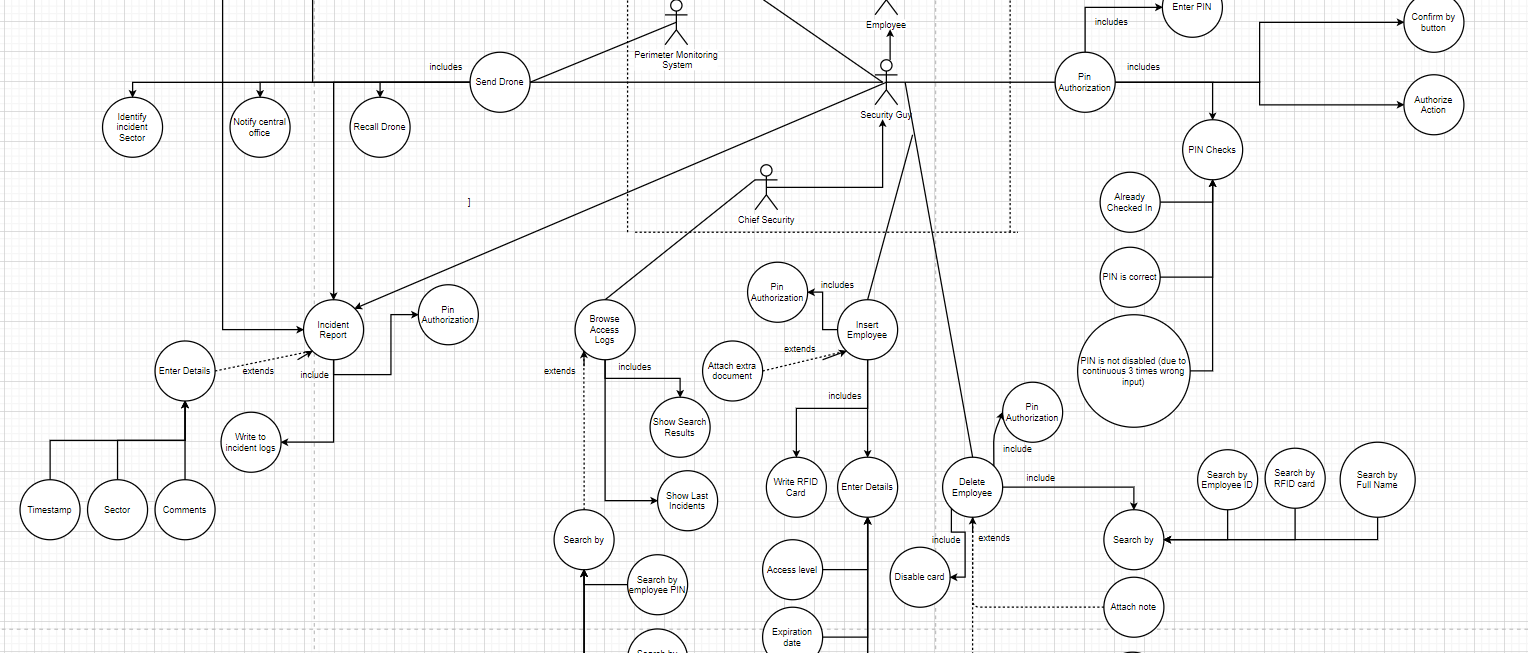
\includegraphics[width=5in]{use2}\\[1ex]\\\\
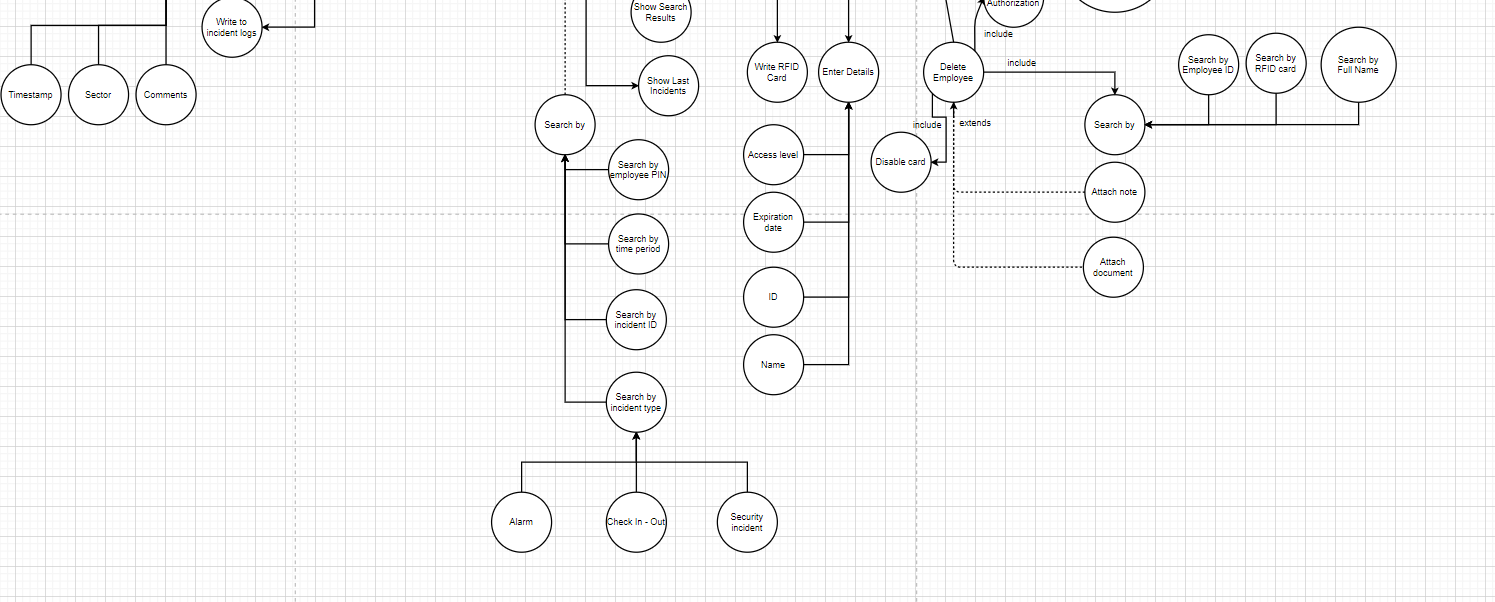
\includegraphics[width=5in]{use3}\\[1ex]\\\\


\section{Εργαλεία}
Χρησιμοποιήθηκαν:
\begin{itemize}
    \item \LaTeX/Overleaf.com - Συγγραφή του παρόντος τεχνικού κειμένου
    \item Photoshop - Φωτογραφία Σελίδας Τίτλου
    \item draw.io - Σχεδιασμός διαγραμμάτων
\end{itemize}


\end{document}
